\documentclass[11pt]{article}
\usepackage[margin=1in]{geometry}
\usepackage{amsmath,amssymb}
\usepackage{enumitem}
\usepackage{hyperref}
\hypersetup{hidelinks}
\setlist{noitemsep}
\usepackage{booktabs}
\usepackage{tabularx}
\usepackage{graphicx}

\title{Architectural Budget Model: Data, Features, Formulas, and Training}
\date{}
\begin{document}
\maketitle

\section*{Process overview (part-by-part)}
\begin{enumerate}[label=Part~\arabic*:, leftmargin=*]
  \item Data acquisition and schema normalization.
  \item Data cleaning and target transformation.
  \item Feature engineering (regex, sums, ratios).
  \item Feature matrix construction (10 inputs).
  \item Polynomial expansion (deg 2) and z-score standardization.
  \item Train/test split (80/20).
  \item Baseline LSBoost training and evaluation.
  \item Feature selection by importance.
  \item Bayesian hyperparameter optimization and final training.
  \item Final evaluation, asset saving, and inference.
\end{enumerate}

\section*{Variables glossary}
\small
\noindent\begin{tabularx}{\textwidth}{@{} l l l l X @{}}
\toprule
Clean name & Source header & Type & Unit & Definition / Role \\
\midrule
project & Project & text & n/a & Project title; used to parse \texttt{num\_storeys}, \texttt{num\_classrooms}. \\
year & Year & numeric & year & Project year; raw feature. \\
budget & Budget & numeric & PHP & Target; filtered $>100{,}000$, then log1p. \\
quantityofplaster\_sq\_m\_\_ & Quantity of plaster (sq.m.) & numeric & sq.m. & Plaster area. \\
quantityofglazedtiles\_sq\_m\_\_ & Quantity of glazed tiles (sq.m.) & numeric & sq.m. & Tiles area. \\
paintingmasonry\_sq\_m\_\_ & Painting masonry (sq.m.) & numeric & sq.m. & Used in total painting. \\
paintingwood\_sq\_m\_\_ & painting wood (sq.m.) & numeric & sq.m. & Used in total painting. \\
paintingmetal\_sq\_m\_\_ & painting metal (sq.m.) & numeric & sq.m. & Used in total painting. \\
areaofchb100mm\_sq\_m\_\_ & Area of CHB 100mm (sq.m.) & numeric & sq.m. & Used in total CHB. \\
areaofchb150mm\_sq\_m\_\_ & Area of CHB 150mm (sq.m.) & numeric & sq.m. & Used in total CHB. \\
num\_storeys & parsed from project & numeric & count & Integer before ``STY''. \\
num\_classrooms & parsed from project & numeric & count & Integer before ``CL''. \\
total\_painting\_area & derived & numeric & sq.m. & paintingmasonry + paintingwood + paintingmetal. \\
total\_chb\_area & derived & numeric & sq.m. & areaofchb100mm + areaofchb150mm. \\
total\_finishes\_area & derived & numeric & sq.m. & plaster + glazed tiles. \\
plaster\_per\_chb & derived & numeric & ratio & plaster / total\_chb\_area; NaN/Inf=0. \\
tiles\_per\_chb & derived & numeric & ratio & glazed tiles / total\_chb\_area; NaN/Inf=0. \\
\bottomrule
\end{tabularx}
\normalsize

\section*{Part 1: Data acquisition and normalization}
Import CSV, clean headers using \verb|makeValidName| and lower-case; drop unnamed columns.

\section*{Part 2: Cleaning and target}
Coerce numeric-like strings, drop NaN budgets, median-impute numeric NaNs. Define $y=\log(1+\text{budget})$ and filter budget $>100{,}000$.

\section*{Part 3: Feature engineering}
Regex on \texttt{project} to obtain \texttt{num\_storeys}, \texttt{num\_classrooms}. Compute \texttt{total\_painting\_area}, \texttt{total\_chb\_area}, \texttt{total\_finishes\_area}, \texttt{plaster\_per\_chb}, \texttt{tiles\_per\_chb}.

\section*{Part 4: Feature matrix (10 inputs)}
$X_{\text{raw}} = [\text{year},\text{num\_storeys},\text{num\_classrooms},\verb|quantityofplaster_sq_m__|,\verb|quantityofglazedtiles_sq_m__|,\text{total\_painting\_area},\text{total\_chb\_area},\text{total\_finishes\_area},\text{plaster\_per\_chb},\text{tiles\_per\_chb}]$.

\section*{Part 5: Polynomial expansion and scaling}
Generate degree-2 squares and pairwise interactions (65 features total), then z-score on training set; NaNs set to 0.

\section*{Part 6: Split}
80/20 holdout via \verb|cvpartition(HoldOut=0.2)|.

\section*{Part 7: Baseline LSBoost}
Train LSBoost (NumLearningCycles=100). Predict on test; invert with \(\exp(\cdot)-1\). Report $R^2$ and MAE.

\section*{Part 8: Feature selection}
Keep features with importance above median (32/65 in the logged run).

\section*{Part 9: Optimized LSBoost}
Bayesian tuning over NumLearningCycles [500,1000], MaxNumSplits [8,32], LearnRate [0.01,0.1] (log scale). Best observed: 714 cycles, 8 splits, lr 0.099656.

\section*{Part 10: Evaluation, assets, inference}
Test metrics (from run): baseline $R^2=0.7993$, MAE $=4{,}416{,}399.93$; optimized $R^2=0.8476$, MAE $=4{,}247{,}884.28$. Assets saved: \verb|optimized_model|, \verb|mu|, \verb|sigma|, \verb|selected_mask|, \verb|final_feature_columns|, \verb|poly_feature_names|. Inference mirrors training: derive features, expand polynomials, z-score, mask, predict in log-space, invert.

\section*{Key figures}
\begin{figure}[h]
  \centering
  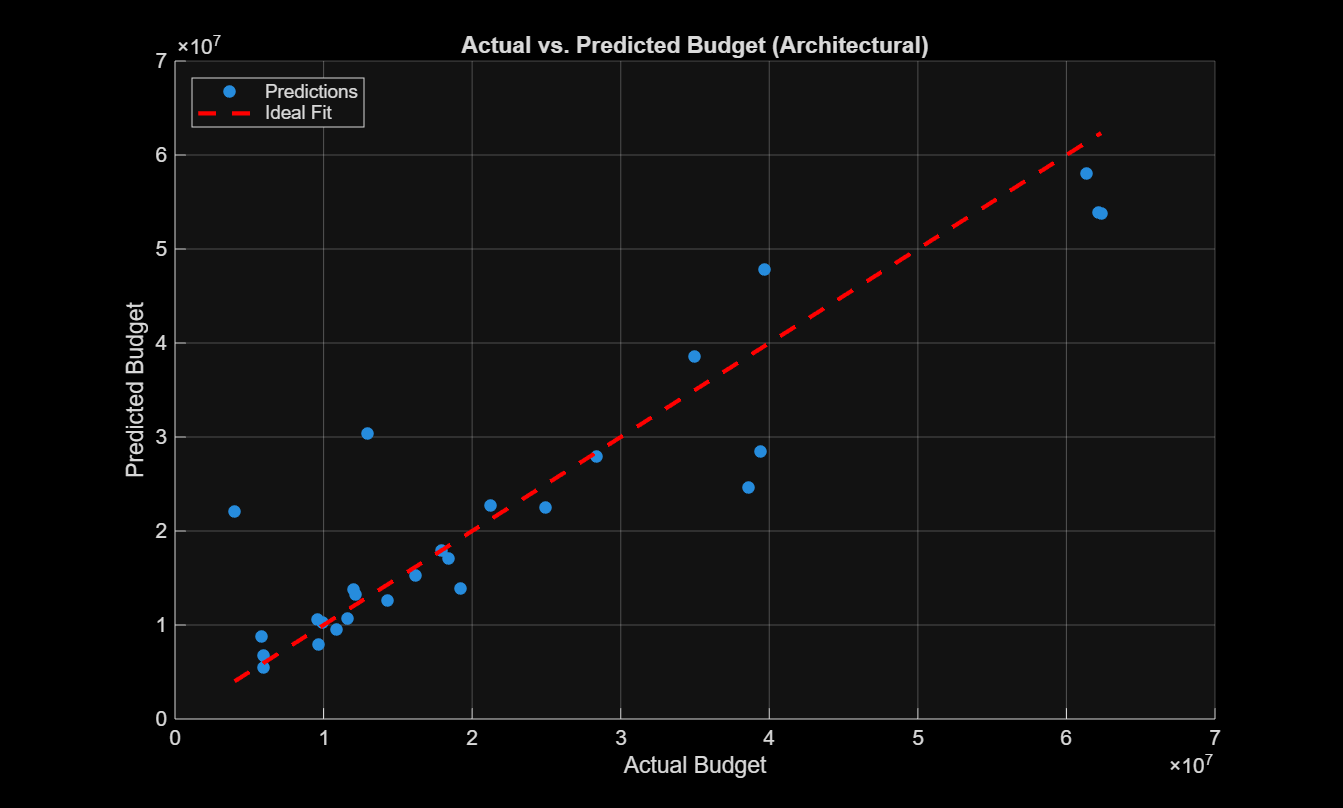
\includegraphics[width=.6\textwidth]{visualizations/actual_vs_predicted_architectural.png}
  \caption{Actual vs. Predicted Budget (Architectural).}
\end{figure}
\begin{figure}[h]
  \centering
  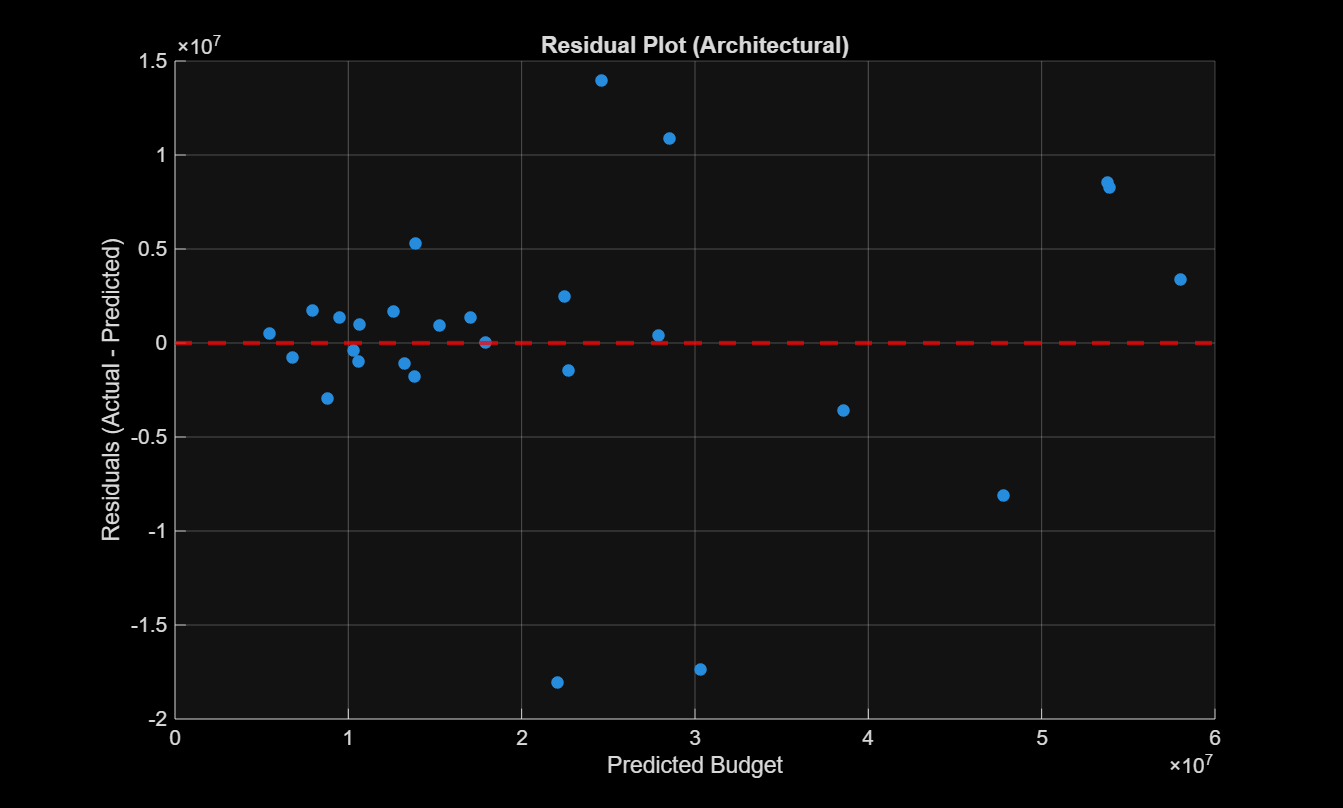
\includegraphics[width=.6\textwidth]{visualizations/residual_plot_architectural.png}
  \caption{Residuals vs. Predicted Budget (Architectural).}
\end{figure}
\begin{figure}[h]
  \centering
  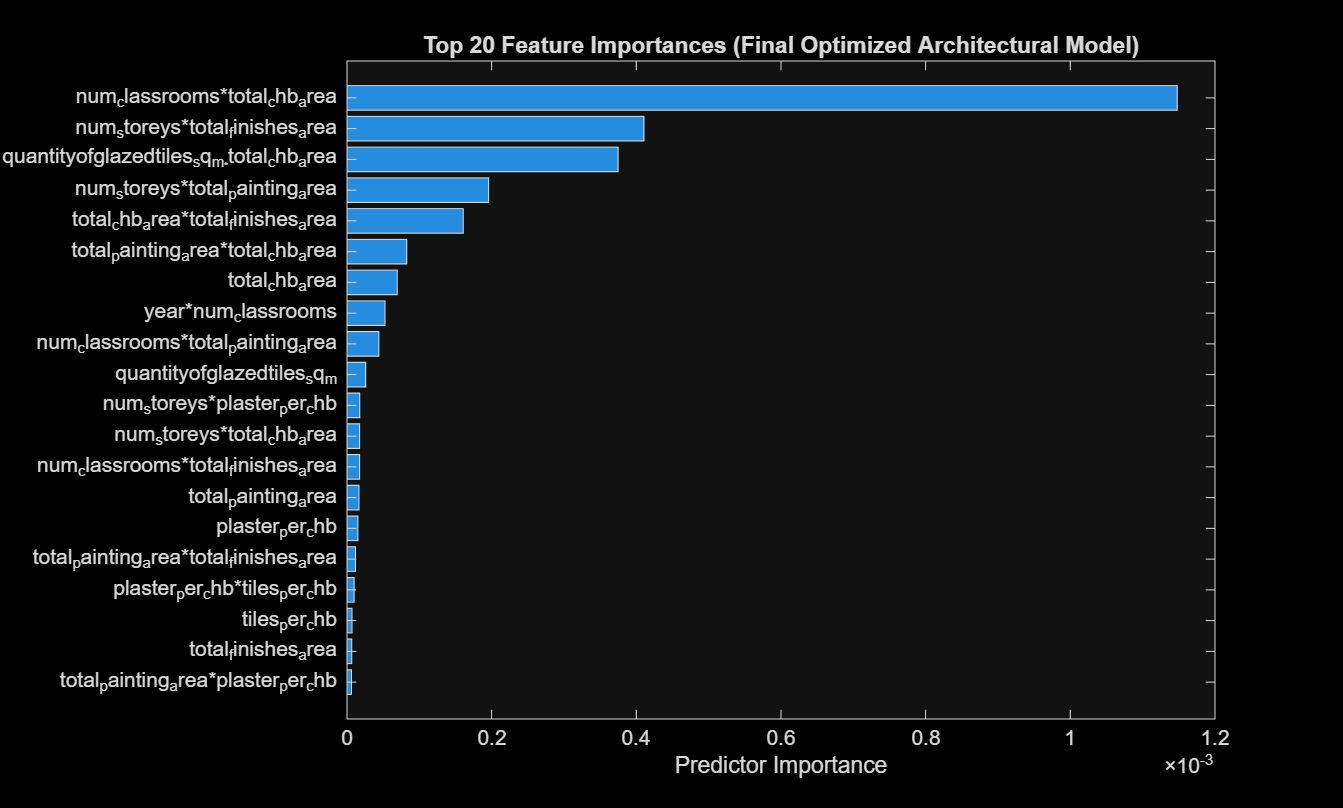
\includegraphics[width=.6\textwidth]{visualizations/feature_importance_final_architectural.png}
  \caption{Top feature importances (optimized ensemble).}
\end{figure}
\begin{figure}[h]
  \centering
  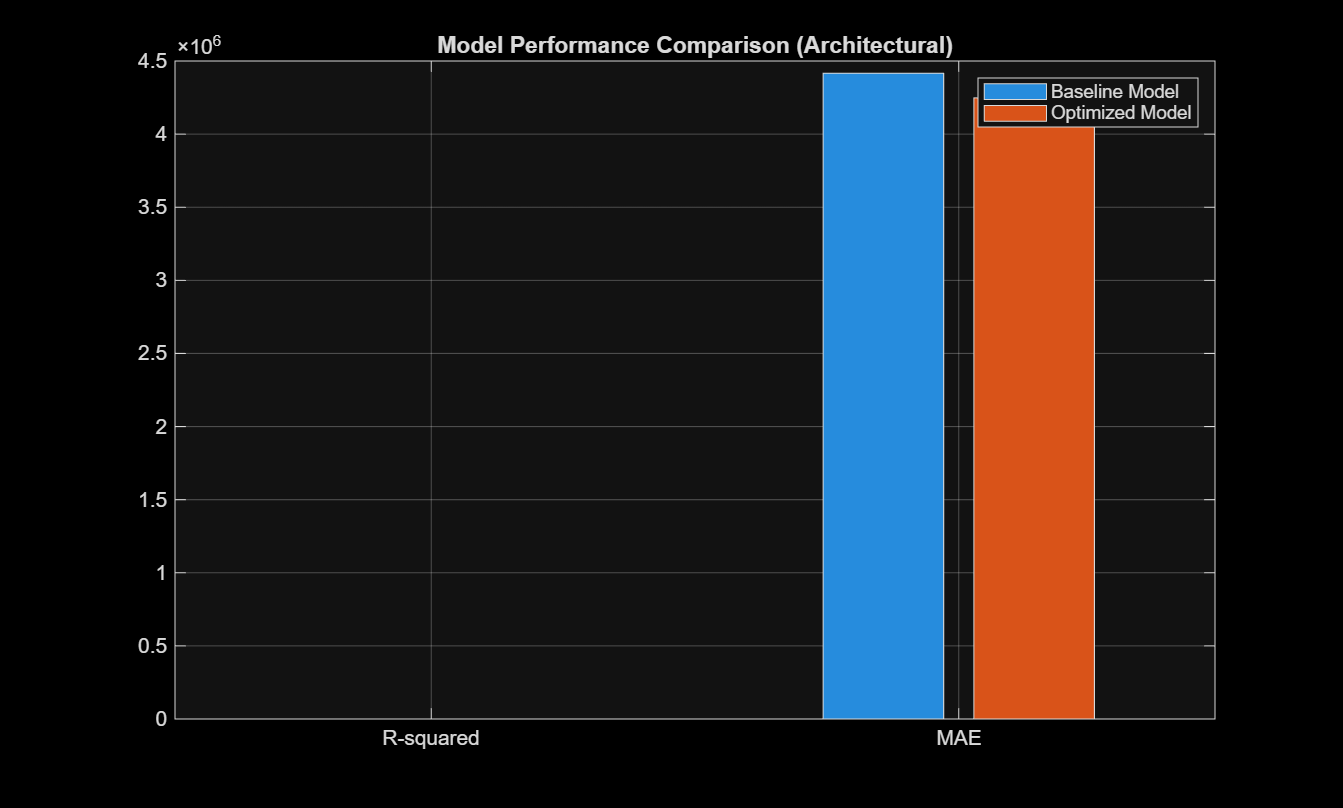
\includegraphics[width=.6\textwidth]{visualizations/performance_comparison_architectural.png}
  \caption{Baseline vs. optimized performance.}
\end{figure}

\section*{Raw data and variables}
Data source: Architectural\_Total\_Cost.csv. Raw columns (pre-clean):
\begin{itemize}
  \item project (text)
  \item year
  \item budget
  \item Quantity of plaster (sq.m.)
  \item Quantity of glazed tiles (sq.m.)
  \item Painting masonry (sq.m.)
  \item painting wood (sq.m.)
  \item painting metal (sq.m.)
  \item Area of CHB 100mm (sq.m.)
  \item Area of CHB 150mm (sq.m.)
\end{itemize}
All headers are cleaned to lower-case MATLAB-valid names; unnamed columns are dropped.

\section*{Exact cleaned variable names (after makeValidName + lower)}
Original CSV headers mapped to cleaned names used in code:
\begin{itemize}
  \item Project $\to$ \verb|project|
  \item Year $\to$ \verb|year|
  \item Budget $\to$ \verb|budget|
  \item Quantity of plaster (sq.m.) $\to$ \verb|quantityofplaster_sq_m__|
  \item Quantity of glazed tiles (sq.m.) $\to$ \verb|quantityofglazedtiles_sq_m__|
  \item Painting masonry (sq.m.) $\to$ \verb|paintingmasonry_sq_m__|
  \item painting wood (sq.m.) $\to$ \verb|paintingwood_sq_m__|
  \item painting metal (sq.m.) $\to$ \verb|paintingmetal_sq_m__|
  \item Area of CHB 100mm (sq.m.) $\to$ \verb|areaofchb100mm_sq_m__|
  \item Area of CHB 150mm (sq.m.) $\to$ \verb|areaofchb150mm_sq_m__|
\end{itemize}

\section*{Cleaning and preprocessing}
\begin{itemize}
  \item Detect and standardize budget column to name \texttt{budget}.
  \item Convert \texttt{budget} and any numeric-like cell strings to numbers (strip commas).
  \item Drop rows with NaN \texttt{budget}.
  \item Median impute all remaining numeric NaNs:
  \[
    x_{ij} \leftarrow 
    \begin{cases}
      x_{ij}, & \text{if not NaN} \\
      \mathrm{median}(x_{\cdot j}), & \text{if NaN}.
    \end{cases}
  \]
  \item Response transformation:
  \[
    y \;=\; \log(1+\mathrm{budget}).
  \]
  \item Filter for training/analysis: \texttt{budget} $> 100{,}000$.
\end{itemize}

\section*{Feature engineering}
From \texttt{project} text using regex, derive:
\[
\text{num\_storeys} := \text{first integer before ``STY''},\quad
\text{num\_classrooms} := \text{first integer before ``CL''}.
\]
Fill missing with column medians.

Auto-detected source columns by substring on cleaned variable names:
\[
\begin{aligned}
&\texttt{plaster\_col} \sim \text{``plaster''},\quad
\texttt{tiles\_col} \sim \text{``glazedtiles''},\\
&\texttt{paintingmasonry},\; \texttt{paintingwood},\; \texttt{paintingmetal},\\
&\texttt{chb100mm},\quad \texttt{chb150mm}.
\end{aligned}
\]
Derived features:
\[
\begin{aligned}
\text{total\_painting\_area} &= \texttt{paintingmasonry} + \texttt{paintingwood} + \texttt{paintingmetal},\\
\text{total\_chb\_area} &= \texttt{chb100mm} + \texttt{chb150mm},\\
\text{total\_finishes\_area} &= \texttt{plaster\_col} + \texttt{tiles\_col},\\
\text{plaster\_per\_chb} &= \frac{\texttt{plaster\_col}}{\text{total\_chb\_area}}\;((\mathrm{NaN/Inf})\rightarrow 0),\\
\text{tiles\_per\_chb} &= \frac{\texttt{tiles\_col}}{\text{total\_chb\_area}}\;((\mathrm{NaN/Inf})\rightarrow 0).\\
\end{aligned}
\]

Final raw feature set used for modeling (in this order):
\[
X_{\text{raw}} = [\,
\text{year},\;
\text{num\_storeys},\;
\text{num\_classrooms},\;
\verb|quantityofplaster_sq_m__|,\;
\verb|quantityofglazedtiles_sq_m__|,\;
\text{total\_painting\_area},\;
\text{total\_chb\_area},\;
\text{total\_finishes\_area},\;
\text{plaster\_per\_chb},\;
\text{tiles\_per\_chb}\,].
\]

\section*{Polynomial/interaction expansion (degree 2)}
Given original features $x_1,\dots,x_p$ from $X_{\text{raw}}$:
\[
X_{\text{poly}} = \big[\, x_1,\dots,x_p,\; x_1^2,\dots,x_p^2,\; x_i x_j\ (1\le i<j\le p)\,\big].
\]
This matches \texttt{generatePolyFeatures(T,2)}.

\section*{Complete polynomial feature name list (65 features)}
For reproducibility, here are the exact feature names emitted by \verb|generatePolyFeatures(T,2)| given the 10 raw features above.

\subsection*{Original 10 features}
\noindent\small
\verb|year|, \verb|num_storeys|, \verb|num_classrooms|, \verb|quantityofplaster_sq_m__|, \verb|quantityofglazedtiles_sq_m__|, \verb|total_painting_area|, \verb|total_chb_area|, \verb|total_finishes_area|, \verb|plaster_per_chb|, \verb|tiles_per_chb|

\normalsize
\subsection*{10 squared features}
\noindent\small
\verb|year^2|, \verb|num_storeys^2|, \verb|num_classrooms^2|, \verb|quantityofplaster_sq_m__^2|, \verb|quantityofglazedtiles_sq_m__^2|, \verb|total_painting_area^2|, \verb|total_chb_area^2|, \verb|total_finishes_area^2|, \verb|plaster_per_chb^2|, \verb|tiles_per_chb^2|

\normalsize
\subsection*{45 pairwise interaction features}
\noindent\small
% year * others (9)
\verb|year*num_storeys|, \verb|year*num_classrooms|, \verb|year*quantityofplaster_sq_m__|, \verb|year*quantityofglazedtiles_sq_m__|, \verb|year*total_painting_area|, \verb|year*total_chb_area|, \verb|year*total_finishes_area|, \verb|year*plaster_per_chb|, \verb|year*tiles_per_chb|,

% num_storeys * next 8
\verb|num_storeys*num_classrooms|, \verb|num_storeys*quantityofplaster_sq_m__|, \verb|num_storeys*quantityofglazedtiles_sq_m__|, \verb|num_storeys*total_painting_area|, \verb|num_storeys*total_chb_area|, \verb|num_storeys*total_finishes_area|, \verb|num_storeys*plaster_per_chb|, \verb|num_storeys*tiles_per_chb|,

% num_classrooms * next 7
\verb|num_classrooms*quantityofplaster_sq_m__|, \verb|num_classrooms*quantityofglazedtiles_sq_m__|, \verb|num_classrooms*total_painting_area|, \verb|num_classrooms*total_chb_area|, \verb|num_classrooms*total_finishes_area|, \verb|num_classrooms*plaster_per_chb|, \verb|num_classrooms*tiles_per_chb|,

% quantityofplaster * next 6
\verb|quantityofplaster_sq_m__*quantityofglazedtiles_sq_m__|, \verb|quantityofplaster_sq_m__*total_painting_area|, \verb|quantityofplaster_sq_m__*total_chb_area|, \verb|quantityofplaster_sq_m__*total_finishes_area|, \verb|quantityofplaster_sq_m__*plaster_per_chb|, \verb|quantityofplaster_sq_m__*tiles_per_chb|,

% quantityofglazedtiles * next 5
\verb|quantityofglazedtiles_sq_m__*total_painting_area|, \verb|quantityofglazedtiles_sq_m__*total_chb_area|, \verb|quantityofglazedtiles_sq_m__*total_finishes_area|, \verb|quantityofglazedtiles_sq_m__*plaster_per_chb|, \verb|quantityofglazedtiles_sq_m__*tiles_per_chb|,

% total_painting_area * next 4
\verb|total_painting_area*total_chb_area|, \verb|total_painting_area*total_finishes_area|, \verb|total_painting_area*plaster_per_chb|, \verb|total_painting_area*tiles_per_chb|,

% total_chb_area * next 3
\verb|total_chb_area*total_finishes_area|, \verb|total_chb_area*plaster_per_chb|, \verb|total_chb_area*tiles_per_chb|,

% total_finishes_area * next 2
\verb|total_finishes_area*plaster_per_chb|, \verb|total_finishes_area*tiles_per_chb|,

% plaster_per_chb * next 1
\verb|plaster_per_chb*tiles_per_chb|

\normalsize

\section*{Scaling}
Compute z-score parameters on training split only:
\[
\mu_j = \frac{1}{n}\sum_{i=1}^n X_{\text{poly},ij},\quad
\sigma_j = \sqrt{\frac{1}{n-1}\sum_{i=1}^n (X_{\text{poly},ij}-\mu_j)^2}.
\]
Scale both train/test:
\[
Z_{ij} = \frac{X_{\text{poly},ij}-\mu_j}{\sigma_j},\quad \text{NaN}\rightarrow 0.
\]

\section*{Train/test split}
Holdout 20\% using \texttt{cvpartition(HoldOut=0.2)}.

\section*{Baseline model}
Least-squares boosting of regression trees:
\[
\hat{f}_{\text{base}} = \mathrm{LSBoost}(Z_{\text{train}},\, y_{\text{train}};\ \text{NumLearningCycles}=100).
\]
Predict on test, invert response:
\[
\hat{y}_{\text{test}}^{(\text{base})} = \exp(\hat{f}_{\text{base}}(Z_{\text{test}})) - 1.
\]

\section*{Feature selection}
Compute importance $I_j$ from the baseline ensemble; select features:
\[
\text{keep}_j \iff I_j > \mathrm{median}(I).
\]
Apply mask to scaled polynomial features to get $Z_{\text{sel}}$.

\section*{Optimized model (final)}
Hyperparameters tuned via Bayesian optimization:
\[
\begin{aligned}
&\text{NumLearningCycles}\in[500,1000]\cap\mathbb{Z},\\
&\text{MaxNumSplits}\in[8,32]\cap\mathbb{Z},\\
&\text{LearnRate}\in[0.01,0.1] \text{ (log scale)}.
\end{aligned}
\]
Train:
\[
\hat{f}_{\star} = \mathrm{LSBoost}(Z_{\text{train,sel}},\ y_{\text{train}};\ \text{optimized HPs}).
\]
Predict and invert:
\[
\hat{y}_{\text{test}} = \exp(\hat{f}_{\star}(Z_{\text{test,sel}})) - 1.
\]

\section*{Evaluation metrics}
With actual budgets $y_{\text{act}}=\exp(y_{\text{test}})-1$ and predictions $\hat{y}$:
\[
R^2 \;=\; 1 - \frac{\sum_i (y_{\text{act},i}-\hat{y}_i)^2}{\sum_i (y_{\text{act},i}-\bar{y}_{\text{act}})^2},
\qquad
\mathrm{MAE} \;=\; \frac{1}{n}\sum_i \lvert y_{\text{act},i}-\hat{y}_i\rvert.
\]

\section*{Saved training assets}
Saved to \texttt{architectural\_model\_assets.mat}:
\[
\{\ \hat{f}_{\star},\ \mu,\ \sigma,\ \text{selected\_mask},\ \text{final\_feature\_columns},\ \text{poly\_feature\_names}\ \}.
\]

\section*{Inference pipeline (single row)}
Given an input row:
\begin{enumerate}
  \item Normalize field names to training names; if needed, auto-compute: \texttt{total\_painting\_area}, \texttt{total\_chb\_area}, \texttt{total\_finishes\_area}, \texttt{plaster\_per\_chb}, \texttt{tiles\_per\_chb}.
  \item Reorder to \texttt{final\_feature\_columns} and build $X_{\text{poly}}$; align by \texttt{poly\_feature\_names}.
  \item Scale: $Z = (X_{\text{poly}}-\mu)/\sigma$, NaN$\rightarrow$0; apply \texttt{selected\_mask}.
  \item Predict log-budget and invert: $\widehat{\mathrm{budget}} \,=\, \exp(\hat{f}_{\star}(Z_{\text{sel}})) - 1$.
\end{enumerate}

\section*{Final list of modeled variables}
Used directly or via derivation:
\[
\begin{aligned}
&\text{year},\ \text{num\_storeys},\ \text{num\_classrooms},\ \verb|quantityofplaster_sq_m__|~(\text{Quantity of plaster (sq.m.)}),\\
&\verb|quantityofglazedtiles_sq_m__|~(\text{Quantity of glazed tiles (sq.m.)}),\ \verb|paintingmasonry_sq_m__|,\\
&\verb|paintingwood_sq_m__|, \verb|paintingmetal_sq_m__|, \verb|areaofchb100mm_sq_m__|, \verb|areaofchb150mm_sq_m__|,\\
&\text{total\_painting\_area},\ \text{total\_chb\_area},\ \text{total\_finishes\_area},\\
&\text{plaster\_per\_chb},\ \text{tiles\_per\_chb},\\
&\text{all degree-2 squares and pairwise interactions of the above 10 raw features.}
\end{aligned}
\]

\end{document}
